Para el análisis de los resultados de la recolección de datos utilizamos
diversos métodos. En primer lugar, tomamos la red como una fuente de
información y las IPs como símbolo. Usando esto como modelo, calculamos la
entropía de las redes invesigadas, usando tanto las ips de los receptores como
las de los emisores de los paquetes ARP. Otro modelo de información posible,
que también nos permitiría caracterizar los nodos de la red y su frecuencia
relativa de aparición, sería utilizar como símbolos las direcciones MAC de los
paquetes. Esto nos da otro tipo de información, porque muchas veces pueden ser
distintos 

Luego, para tener una mejor visualización de los datos obtenidos, decidimos
utilizar diferentes gráficos para sintetizar y presentar la información que
consideramos más relevante de las redes analizadas.

En primer lugar usamos gráficos de torta para representar la proporción de
apariciones entre las IPs, tanto de emisores como receptores. Sin embargo,
cuando el número de IPs distintas crecía (en particular con las redes de la
facultad) este método dejaba de ser eficiente porque el gráfico se volvía
incomprensible. Es por esto que en el caso de las capturas de la facultad
mostramos una versión ``reducida'' del gráfico, con los paquetes de los
primeros 5 minutos en lugar de los 60 que duró la captura.

En segundo lugar, usamos gráficos de barras para analizar la frecuencia
absoluta y relativa de aparición de cada una de las IPs, contando por separado
los paquetes en los que la IP era emisora y receptora.

Por último, usamos un histograma en 2 dimensiones con una escala cromática
que indica la cantidad de veces que la IP de la fila $x$ envió un ARP
preguntando por la IP de la columna $y$.

Para ahorrar espacio con el texto de los gráficos, en todos los casos salvo los
gráficos de torta las IPs se expresan incompletas (solo los últimos 8 bits, que
son los que cambian). La primera parte en el caso de los laboratorios de la
facultad es siempre ``10.2.100'' y en la del trabajo de nuestro compañero
``10.10.99''.

Los resultados y análisis se exponen a continuación.

\subsection{Laboratorios del DC}
Con un total de 200 paquetes ARP capturados, obtuvimos una entropía en los
emisores de 2.81763365265 y en los receptores de 4.20465276111.

\begin{figure}[!h]
  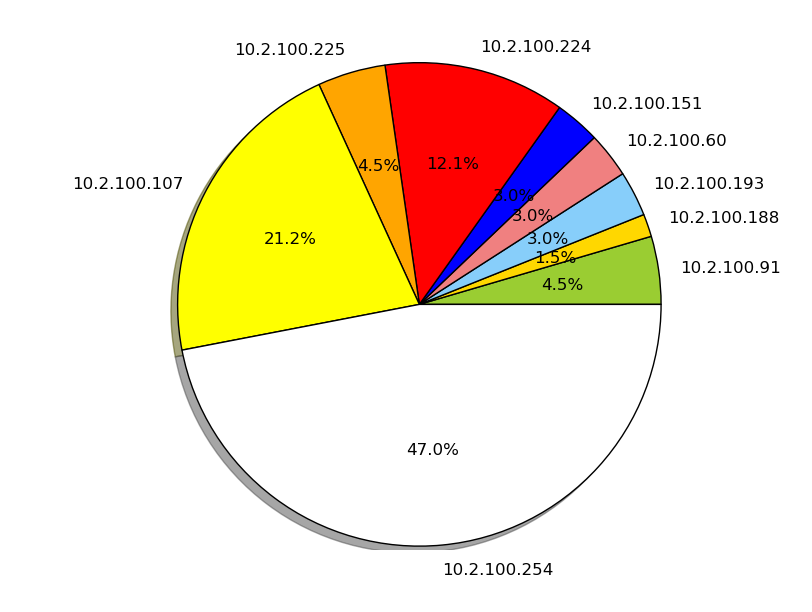
\includegraphics[width=\textwidth,keepaspectratio]{graph/torta-facu.png}
  \caption{Proporción de IPs de los primeros 5 minutos de captura}
  \label{fig:torta-facu}
\end{figure}

\begin{figure}[!h]
  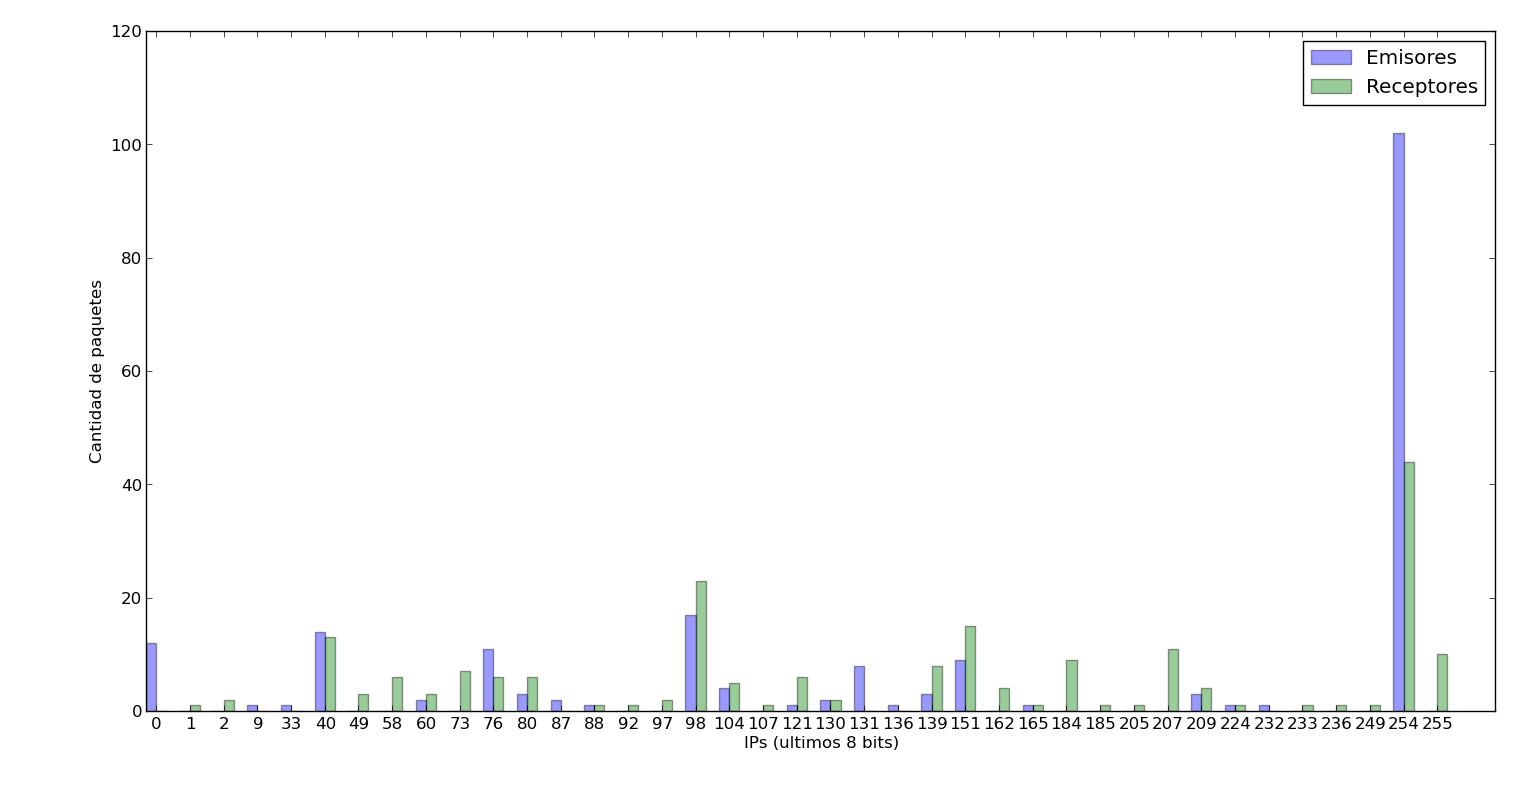
\includegraphics[width=\textwidth,keepaspectratio]{graph/barras-facu.png}
  \caption{Cantidad de paquetes por IP discriminados en emisores y receptores}
  \label{fig:barras-facu}
\end{figure}

\begin{figure}[!h]
  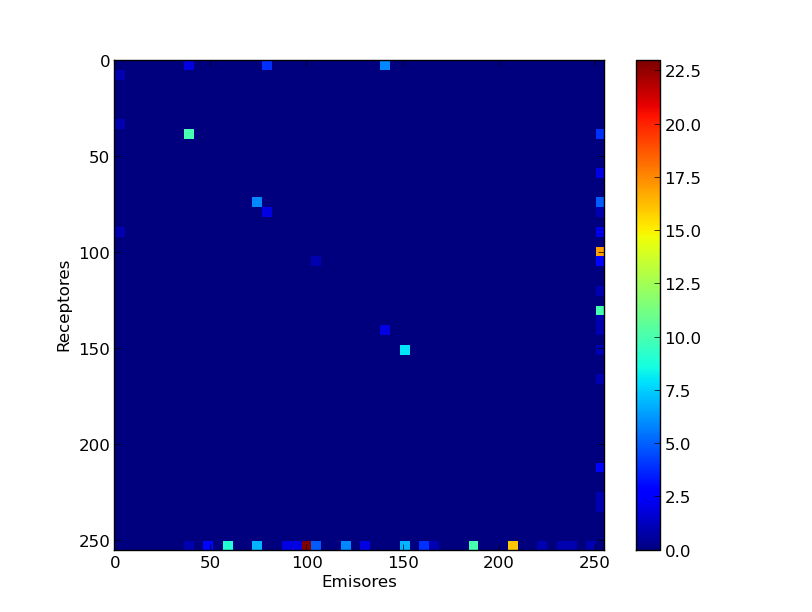
\includegraphics[width=\textwidth,keepaspectratio]{graph/hist2d-facu.png}
  \caption{Relación entre emisores y receptores}
  \label{fig:hist2d-facu}
\end{figure}

Como se puede observar claramente en las figuras \ref{fig:torta-facu} y 
\ref{fig:barras-facu}, hay una gran presencia del dispositivo con la IP
10.2.100.254 (que genera muchas más solicitudes de las que responde),
seguido de lejos por la 10.2.100.98.

Esto también se puede apreciar en la figura \ref{fig:hist2d-facu}, donde se
aprecia que 10.2.100.98 prácticamente solo pregunta por 10.2.100.254.
También en el histograma en se puede visualizar que 10.2.100.254 pregunta por
varias IPs distintas y también es consultado por varias otras. Otra observación,
bastante extraña por cierto, es que hay cierta tendencia de algunos dispositivos
a preguntar por ellos mismos (por eso la clara diagonal del histograma).

En las figuras \ref{fig:barras-facu} y \ref{fig:hist2d-facu} se observa
que la mayor parte de las IPs disponibles (tomando en cuenta solo las que
comienzan por ``10.2.100'') fueron usadas en algún momento de la captura.

En contadas ocasiones (apreciables tanto en el dump de la captura
como en las figuras \ref{fig:barras-facu} y \ref{fig:hist2d-facu}), apareció la
IP 0.0.0.0 (la única que no comienza con ``10.2.100'') como emisora de
solicitudes ARP con distintos destinos. Investigando un poco, descubrimos que
esta es una IP que se utiliza para dispositivos que no están conectados a
ninguna red TCP/IP. Es también una IP ficticia que se usa para representar
direcciones inválidas, a menudo impresoras mal configuradas, paquetes con emisor
desconocido, o cuando DHCP falla o tarda demasiado tiempo.

También descubrimos que, salvo por las consultas autorreferenciales y las que
involucran a 10.2.100.254 y a 0.0.0.0, las consultas entre nodos distintos son
inexistentes.

A raíz de estas observaciones, podemos concluir algunas cosas:
\begin{itemize}
  \item El router de la red seguramente se encuentra en 10.2.100.254, y
probablemente sea el nodo de salida a Internet.
  \item En 10.2.100.98 probablemente haya un dispositivo que estaba configurado
para renovar sus tablas ARP en intervalos cortos.
  \item Hay ocasiones en las que DHCP falla y deja dispositivos sin IP, o bien
hay dispositivos enviando paquetes con IPs emisoras inválidas o secretos. En
cualquier caso, esto arruina la función de ARP, ya que nadie puede
responder a una IP que no es ruteable.
  \item Por momentos los dispositivos tienen leves síntomas de
esquizofrenia.
  \item Más allá de las preguntas por sí mismos y las consultas al router, no
existen consultas entre dispositivos. Mientras duró la captura ninguno de ellos
trató de comunicarse con otro.
  \item Todo esto nos lleva a pensar que la función principal de la red es
proveer de salida a Internet a los dispositivos que se conecten a ella, más que
permitirles la comunicación directa entre dispositivos de la misma red.
  \item La cantidad de dispositivos conectados a la red es grande.  Esto podría
explicar la sobrecarga del servidor de DHCP, que falla o tarda mucho tiempo en
asignar IPs a los nuevos dispositivos. 
\end{itemize}

\newpage
\subsection{Oficinas de InvGate}
Con un total de 11158 paquetes ARP capturados, obtuvimos una entropía en los
emisores de 2.85760098357 y en los receptores de 3.08636573523.

\begin{figure}[!h]
  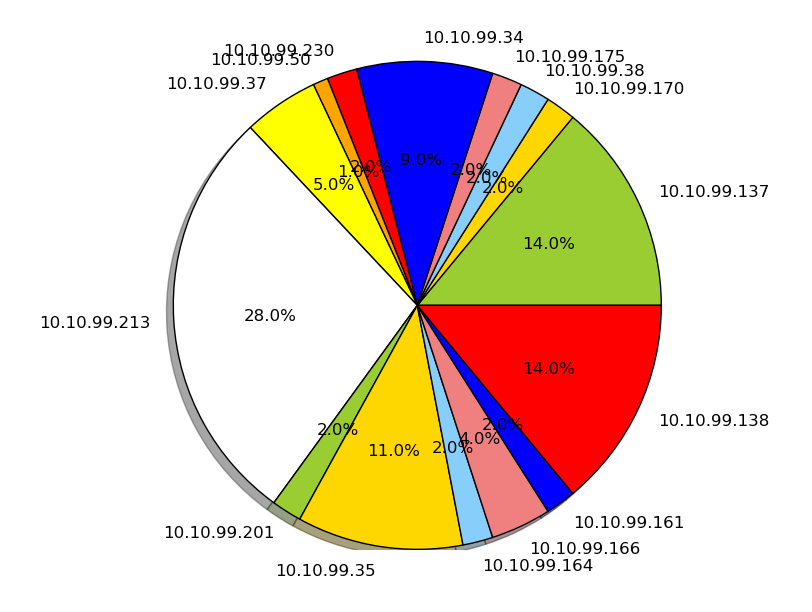
\includegraphics[width=\textwidth,keepaspectratio]{graph/torta-invgate.png}
  \caption{Proporción de la aparición de las IPs en las capturas.}
  \label{fig:torta-inv}
\end{figure}

\begin{figure}[!h]
  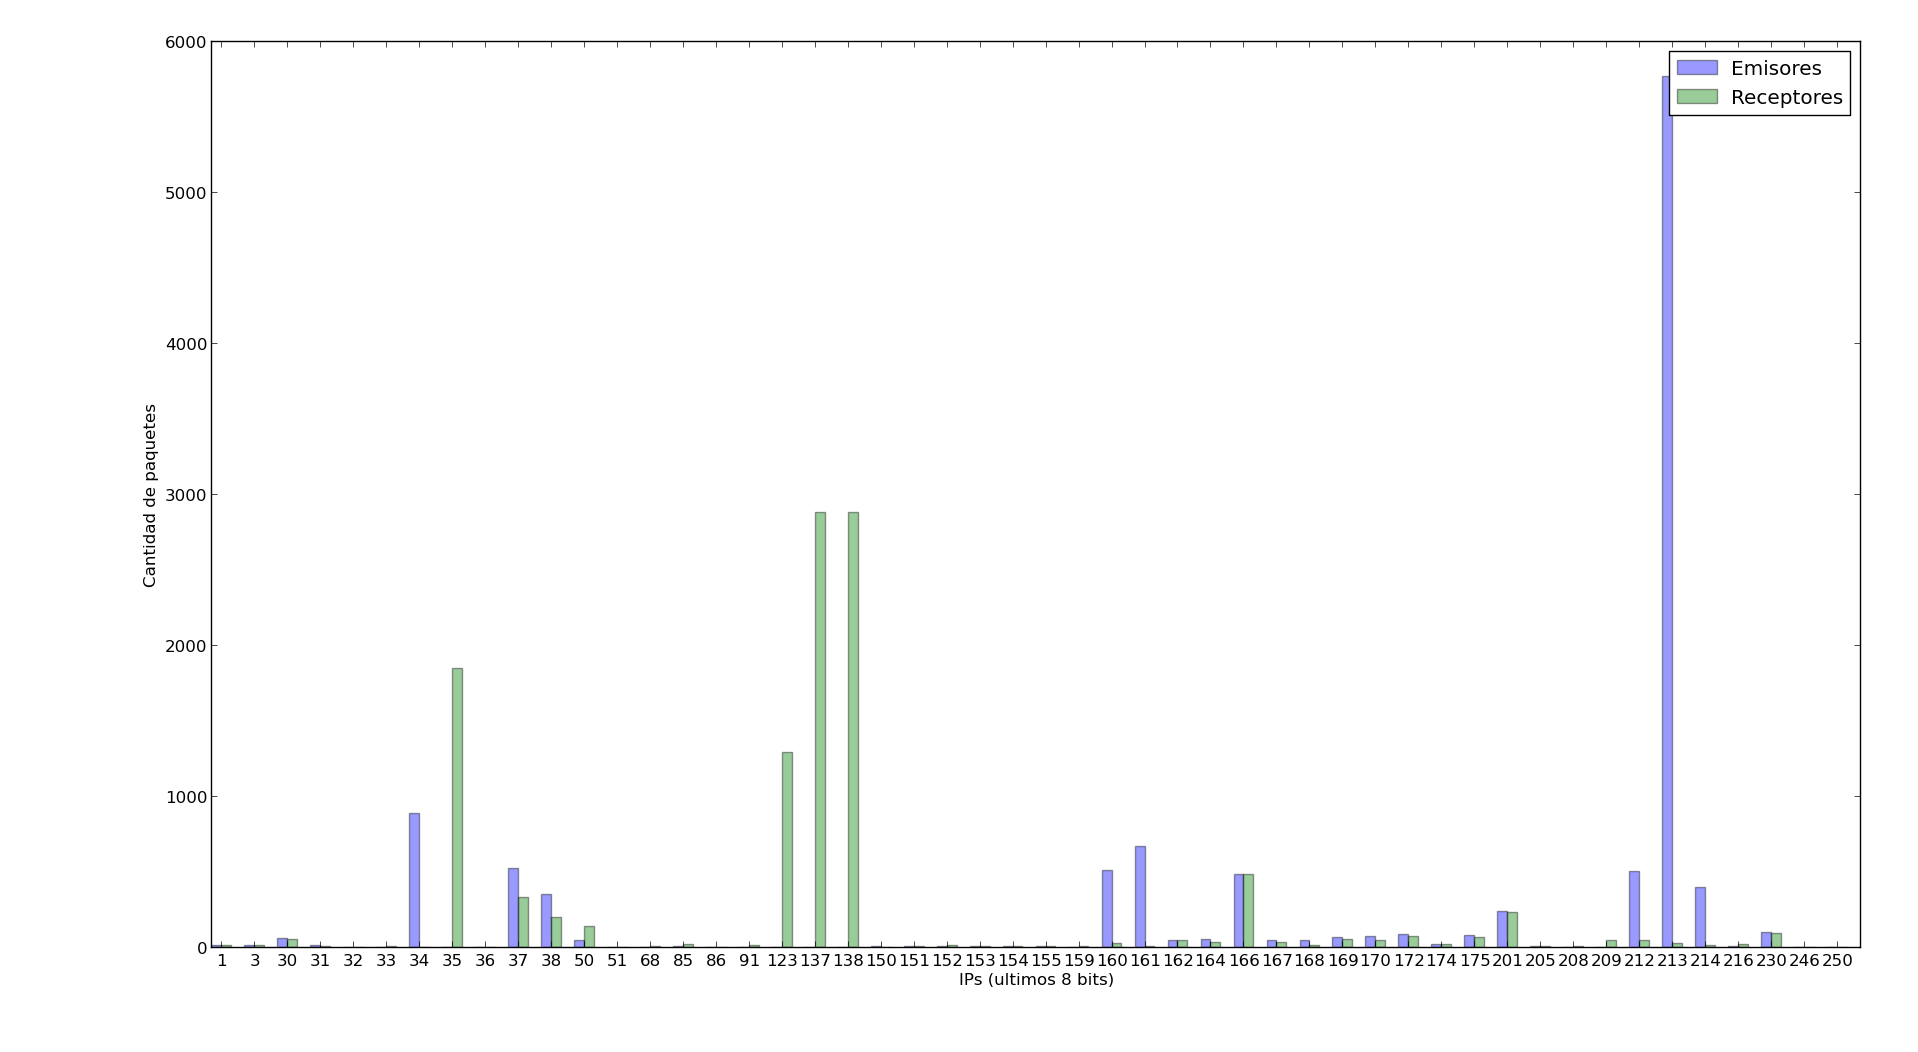
\includegraphics[width=\textwidth,keepaspectratio]{graph/barras-invgate.png}
  \caption{Cantidad de paquetes por IP discriminados en emisores y receptores}
  \label{fig:barras-inv}
\end{figure}

\begin{figure}[!h]
  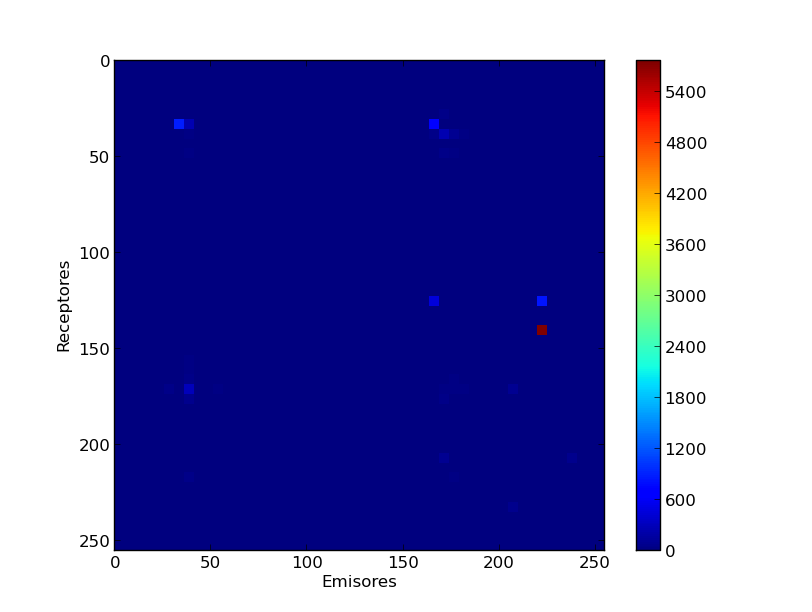
\includegraphics[width=\textwidth,keepaspectratio]{graph/hist2d-invgate.png}
  \caption{Relación entre emisores y receptores}
  \label{fig:hist2d-inv}
\end{figure}

Como se puede observar claramente en las figuras \ref{fig:torta-inv} y 
\ref{fig:barras-facu}, hay una gran presencia del dispositivo con la IP 10.10.99.213 cuyo comportamiento se limita a generar paquetes ARP y envíarlos, nunca es el destino de una consulta who-is. Por otro lado, a éste lo siguen dos dispositivos que tienen la misma cantidad de apariciones en los paquetes: las IPs 10.10.99.138 y 10.10.99.137. En las capturas, estos dos dispositivos se encuentran siempre como IPs destino, es decir, IPs por las cuales se consulta o se informa a qué MAC corresponde.
 
En la figura \ref{fig:hist2d-facu} podemos ver la interacción que se corresponde con estos dispositivos. Vemos que casi la totalidad de los paquetes envíados por el dispositivo 213 están dirigidos a los dispositivos 137, 138 o 123. 	
También en el histograma se puede visualizar las peticiones que recibe el dispositivo 35, que ya podíamos ver en el gráfico de barras era receptor de varios paquetes. Pregunta por
varias IPs distintas y también es consultado por varias otras.

En las figuras \ref{fig:barras-facu} y \ref{fig:hist2d-facu} se observa
que la mayor parte de las IPs disponibles (tomando en cuenta solo las que
comienzan por ``10.2.100'') fueron usadas en algún momento de la captura.

En contadas ocasiones (apreciables tanto en el dump de la captura
como en las figuras \ref{fig:barras-facu} y \ref{fig:hist2d-facu}), apareció la
IP 0.0.0.0 (la única que no comienza con ``10.2.100'') como emisora de
solicitudes ARP con distintos destinos. Investigando un poco, descubrimos que
esta es una IP que se utiliza para dispositivos que no están conectados a
ninguna red TCP/IP. Es también una IP ficticia que se usa para representar
direcciones inválidas, a menudo impresoras mal configuradas, paquetes con emisor
desconocido, o cuando DHCP falla o tarda demasiado tiempo.

También descubrimos que, salvo por las consultas autorreferenciales y las que
involucran a 10.2.100.254 y a 0.0.0.0, las consultas entre nodos distintos son
inexistentes.

A raíz de estas observaciones, podemos concluir algunas cosas:
\begin{itemize}
  \item El router de la red seguramente se encuentra en 10.2.100.254, y
probablemente sea el nodo de salida a Internet.
  \item En 10.2.100.98 probablemente haya un dispositivo que estaba configurado
para renovar sus tablas ARP en intervalos cortos.
  \item Hay ocasiones en las que DHCP falla y deja dispositivos sin IP, o bien
hay dispositivos enviando paquetes con IPs emisoras inválidas o secretos. En
cualquier caso, esto arruina la función de ARP, ya que nadie puede
responder a una IP que no es ruteable.
  \item Por momentos los dispositivos tienen leves síntomas de
esquizofrenia.
  \item Más allá de las preguntas por sí mismos y las consultas al router, no
existen consultas entre dispositivos. Mientras duró la captura ninguno de ellos
trató de comunicarse con otro.
  \item Todo esto nos lleva a pensar que la función principal de la red es
proveer de salida a Internet a los dispositivos que se conecten a ella, más que
permitirles la comunicación directa entre dispositivos de la misma red.
  \item La cantidad de dispositivos conectados a la red es grande.  Esto podría
explicar la sobrecarga del servidor de DHCP, que falla o tarda mucho tiempo en
asignar IPs a los nuevos dispositivos. 
\end{itemize}

